\documentclass{article}

\usepackage[utf8]{inputenc}
\usepackage{graphicx}
\usepackage{listings}


\renewcommand{\contentsname}{Contenidos}

\title{Esborrany Treball de Recerca:\\Teoría e implementación de un motor gráfico}
\date{Curso 2017/2018}
\author{Alumno: Joel Pérez\\Profesor: José Ramírez\\Departamento de Matemáticas}


\begin{document}
\lstset{language=C, basicstyle=\ttfamily}
\pagenumbering{gobble}

\maketitle


\newpage

\pagenumbering {arabic}

\tableofcontents

\newpage



\section{Resumen del trabajo}
\subsection{Introducción}
En la actualidad están apareciendo multitud de herramientas cuyo objetivo es ahorrar tiempo al usuario en el proceso de producción. En mi opinión, el sector que más está experimentando este cambio es el mismo proceso de desarrollo de software. Además de la aparición de entornos que abarcan todos los pasos del proceso de creación de software (IDE) están apareciendo motores gráficos que agilizan en gran medida la creación de videojuegos, eliminando un laborioso proceso que podía llegar a ocupar años, la elaboración de un motor gráfico....
\newline
La llegada de esta ola de software que pretende agilizar el desarrollo ha sido bastante polémica. Por una parte no se puede negar la importancia de tener herramientas más potentes. Pero por la otra parte hay muchos que piensan que esto ha llevado a la gente a no preocuparse por algunas cuestiones sólo porque lo ven como una cosa del pasado, un problema menor. Estos problemas terminan por acumularse y pueden desencadenar en problemas mayores si no se intentan solventar desde la raíz.
\subsection{Objetivos}
El objetivo de este trabajo consiste en investigar la factibilidad de desarrollar un motor gráfico utilizando herramientas relativamente simples. El objetivo de la investigación no es crear un motor gráfico comercial dada tanto la limitación tanto de conocimientos como de tiempo. Se pretende estudiar cómo funciona a nivel interno un motor, para poder determinar si realmente es interesante crear un motor gráfico propio para cada proyecto dependiendo de las características del mismo o si realmente deberíamos de utilizar motores gráficos comerciales.
\newline
Para ello se intentará hacer una implementación primero sin OpenGL y compararla con una con OpenGL para intentar notar las diferencias en cuanto a rendimiento. Posteriormente se intentará buscar un motor gráfico comercial para compararlo con los primeros dos motores. Contra más funcionalidad comparta el motor gráfico ``hecho a mano'' con el comercial, más cerca nos acercaremos de desarrollar una conclusión realista.
\subsection{Motivación personal}
Existen una gran cantidad de motivaciones personales alrededor de este proyecto. Por una parte soy un gran fanático de la computación y con el Treball de Recerca tengo una buena oportunidad de hacer algo que siempre he deseado hacer. También me he inspirado por un videojuego llamado ``Handmade hero'', el cuál está siendo desarrollado, como dice el nombre ``a mano'', sin hacer uso de liberías modernas. También tengo interés es aprender a hacer un programa de un tamaño más grande de lo que estoy acostumbrado y de aprender a documentar todo el proceso, además de aprender a usar diversas herramientas para redactar textos científicos.
\subsection{Relevancia del estudio en el campo}
Como he comentado previamente, en la actualidad existe una gran polémica con respecto a este tema. Muchas empresas de la indústria de los videojuegos han decidido abandonar la creación de motores para uso específico de sus videojuegos en pro de adoptar motores comerciales generales. Esta decisión puede traer muchos problemas debido a la extrema complejidad de los juegos modernos, que requiere de un motor que esté adaptado a las necesidades específicas del videojuego.
\newline
Ser capaz de entender el funcionamiento de un motor gráfico debería de poder ayudar a tomar la decisión, y definitivamente creo que ayuda a ser más eficiente a la hora de trabajar con el motor en sí, sea uno ``hecho a mano'' o uno general.
\subsection{Límites del trabajo}
Está clara la inviabilidad de desarrollar un motor gráfico a la altura de los ofrecidos actualmente en el mercado, pues estos están desarrollados por un equipo de expertos y tienden a ofrecer una cantidad de funcionalidad que duramente se puede replicar en un proyecto hecho en unos meses por alguien que no tiene la formación necesaria.
\subsection{Metodología empleada para realizar la investigación}
El método de trabajo consiste en la creación de un motor gráfico con una funcionalidad limitada pero suficiente para intentar elaborar una conclusión. Este motor gráfico se utilizará para hacer demostraciones y ejemplificar las operaciones que ocurren en un motor gráfico moderno.
\section{Planteamiento de la hipótesis}
Tengo la hipótesis de que los equipos de desarrollo de software deberían de aspirar a ser ellos mismos quienes crean las herramientas que utilitzarán para crear el software en sí. En caso de que esta sea una decisión no rentable, su máxima prioridad debería de ser entender cómo funcionan las herramientas que utilizarán. Considero que cuando uno forma parte en el proceso de creación de software, tiene que tener un conocimiento total o mayoritario del funcionamiento de aquello que está haciendo. Eso signfica pasar por pasos que muchas veces se saltan con la finalidad de agilizar el proceso, no obstante no creo que esto sea positivo ya que ha llevado a serios problemas a la larga.
\newpage
\section{Previsión del índice}
\begin{enumerate}
\item{Introducción al trabajo y hipótesis}\\
  En este apartado se hará una introducción al Treball de Recerca de forma similar a la que se ha hecho en este documento.
\item{Definición de conceptos previos}\\
  Previamente a la lectura del documento se familirizará al lector con concpetos que considero necesarios para la comprensión del mismo. Ejemplo: tecnicismos, conceptos matemáticos...
\item{Teoría de un motor gráfico}\\
  En esta sección se comentará sobre la funcionalidad de un motor gráfico a nivel teórico, sin entrar a consideraciones técnicas, se hablará de los distintos tipos de operaciones que utiliza.
\item{Implementación de un motor gráfico}\\
  Una vez estudiados los conceptos teóricos se expondrá cómo se han implementado. Se entrará en detalle sobre las decisiones de tipo técnico que se han usado.
\item{Estudio de la situación actual}\\
  Mi objetivo es intentar contactar con principales apologistas de la importancia de conocer el software con el que trabaja uno y intentar recopilar sus opiniones en esta sección.
\item{Valoración general y conclusión}\\
  Finalmente, utilizando las nociones aprendidas en el transcurso de este Treball de Recerca se intentará llegar a una conclusión y ver si la hipótesis presentada realmente se sostiene tras finalizar el trabajo.
\end{enumerate}

\newpage
\section{Ejemplo de la expresión del documento final}
\subsection{Definición de un punto}
Un punto es una figura geométrica sin dimensión, tampoco tiene longitud, área, volumen, ni otro ángulo dimensional. No es un objeto físico. Describe una posición en el espacio, determinada respecto de un isstema de coordenadas preestablecidas.
\subsection{Definición de un punto en el programa}
\begin{lstlisting}[frame=single]
  struct Point 
  float x;          // Coordenada 'x'
  float y;          // Coordenada 'y'
  float z;          // Coordenada 'z'
  float w;          // w = 1 si el punto es un vector
  };
  
\end{lstlisting}

\subsection{Definición de un cubo}
Un cubo o hexaedro regular es un poliedro limitado por seis caras cuadradas congrugentes. El cubo tiene seis caras, ocho vertices y doce aristas.
\begin{center}
  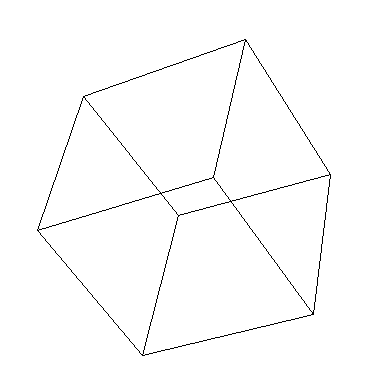
\includegraphics[scale=0.5]{img/cube.png}
\end{center}
\subsection{Definición de un cubo en el programa}
\begin{lstlisting}[frame=single]
  struct Cube {
    Point P[8];
  };
\end{lstlisting}
\subsubsection{Operación del cubo: Traslación}
Una traslación desplaza cada punto de una figura o espacio a la misma cantidad en una determinada dirección. Actualmente en el programa sólo se puede desplazar un cubo en uno de los tres ejes con un valor determinado. Es posible desplazarlo en diferentes ejes utilizando una combinación de traslaciones de un solo eje. \newline
La función acepta un puntero al cubo que se quiere trasladar, por lo que se modifican directamente las coordenadas de los puntos. También acepta un valor que determina el eje sobre el que se trasladará. Y finalmente acepta un valor por el que se trasladará.
\begin{lstlisting}[frame=single]
void translate_cube(Cube *cube, int axis, float value)
{
  for (int i = 0; i < 8; ++i){
    switch (axis){
    case AXIS_X:
      cube->P[i].x += value;
      break;
    case AXIS_Y:
      cube->P[i].y += value;
      break;
    case AXIS_Z:
      cube->P[i].z += value;
      break;
    }
  }
}
\end{lstlisting}


\end{document}

